\documentclass[12pt, letterpaper]{article}

% ==========================================
%              DOCUMENT PACKAGES
% ==========================================

% --- Core Language & Encoding ---
\usepackage[english]{babel} % Sets the language and regional settings for English documents
\usepackage[utf8]{inputenc} % Allows the use of UTF-8 characters in the document
\usepackage[T1]{fontenc} % Specifies the font encoding
\usepackage[margin=2cm]{geometry} % Sets the page margins

% --- Colors & Graphics ---
\usepackage[table,dvipsnames]{xcolor} % Advanced color management
% \usepackage{color} % Basic package for text and background colors
\usepackage{graphicx} % Enhanced support for including external images and scaling them
\usepackage{adjustbox} % Adjusts the size, scaling, and alignment of boxes, images, and tables
% \usepackage{background} % Allows adding background images or watermarks to pages
\usepackage{float} % Improves the interface for floating objects and adds the [H] placement
\usepackage{pdflscape} % Makes landscape pages display correctly on screen in PDF viewers
\usepackage{pdfpages} % Allows the inclusion of external multi-page PDF documents

% --- Math, Science & Engineering ---
\usepackage{amsfonts} % Provides extended mathematical fonts
\usepackage{amsmath} % Provides advanced mathematical typesetting and environments
\usepackage{amssymb} % Provides extended mathematical symbols
% \usepackage{amsmath, amssymb} % (Redundant combination line omitted for stability)
\usepackage{amsthm} % Facilitates the creation of theorem-like environments
\usepackage{mathtools} % Enhances amsmath with additional math tools and bug fixes
\usepackage{thmtools} % Extensions and customization options for theorem environments
\usepackage{nicematrix} % Enhances matrices and tabulars using PGF/TikZ
\usepackage{xy} % Typesets complex graphs and diagrams
\usepackage{circuitikz} % Allows drawing of electrical networks and circuits

% --- Typography & Fonts ---
\usepackage{avant} % Sets the default sans-serif font to Avant Garde
\usepackage{cantarell} % Sets the default sans-serif font to Cantarell
\usepackage{charter} % Sets the default roman font to Charter
\usepackage{cmbright} % Sets the font family to Computer Modern Bright 
\usepackage{helvet} % Sets the default sans-serif font to Helvetica
\usepackage{inconsolata} % Sets the default typewriter (monospace) font to Inconsolata
\usepackage{iwona} % Sets the font family to Iwona 
\usepackage{kurier} % Sets the font family to Kurier 
\usepackage{lmodern} % Loads the Latin Modern fonts 
\usepackage{textcomp} % Provides additional text symbols
\usepackage{ulem} % Provides various types of text underlining and strikethroughs

% --- Tables & Lists ---
\usepackage{array} % Extends the array and tabular environments
% \usepackage{arydshln} % Conflicts with longtable
\usepackage{bigstrut} % Adds custom vertical space in table rows
\usepackage{booktabs} % Enhances the quality of tables with better horizontal rules
% \usepackage{colortbl} % Allows coloring of rows, columns, and individual cells in tables
\usepackage{diagbox} % Creates table cells with diagonal lines 
\usepackage{enumitem} % Provides advanced control over list environments
\usepackage{longtable} % Allows tables to break across multiple pages
\usepackage{multirow} % Allows individual table cells to span across multiple rows
\usepackage{tabularx} % Creates tables with dynamically adjustable-width columns
\usepackage{pgfplotstable} % Reads and cleanly formats numerical tables directly from CSV

% --- Formatting, Layout & UI ---
\usepackage{blindtext} % Generates dummy text for testing document layouts
\usepackage{caption} % Customizes captions in floating environments
\usepackage{comment} % Allows you to block out large sections of text
\usepackage{emptypage} % Automatically removes headers and footers on empty pages
\usepackage{fancyhdr} % Allows complete customization of headers and footers
\usepackage{fancyvrb} % Enhanced verbatim environments for writing raw code
\usepackage{framed} % Creates framed, shaded, or differently highlighted text regions
\usepackage{fullpage} % Quickly sets all page margins to 1 inch
\usepackage{lipsum} % Generates Lorem Ipsum dummy text
\usepackage{mdframed} % Creates highly customizable framed environments
\usepackage{multicol} % Allows intermixing single and multiple text columns
\usepackage{parskip} % Replaces standard paragraph indentation with vertical spacing
\usepackage{setspace} % Controls line spacing (single, one-and-a-half, double)
\usepackage{subcaption} % Supports sub-figures and sub-tables with independent captions
% \usepackage{subfig} % Older package for sub-figures (subcaption is generally preferred now)
\usepackage{tcolorbox} % Creates heavily customized colored and framed text boxes
\usepackage{titlesec} % Customizes the formatting of section, subsection, and chapter headings
\usepackage{titling} % Provides advanced control over the typesetting of the document title

% --- Bibliographies & References ---
\usepackage{biblatex} % Advanced, modern bibliographic processing and formatting
\usepackage{csquotes} % Context-sensitive quotation facilities
\usepackage{makeidx} % Supports the generation of a document index
% \usepackage{natbib} % Flexible bibliography support, particularly for author-year citation styles

% --- TikZ & Plotting ---
\usepackage{tikz} % Advanced package for creating vector graphics and diagrams programmatically
\usepackage{pgf-pie} % Draws pie charts programmatically using PGF/TikZ
\usepackage{pgfplots} % Creates high-quality mathematical plots, charts, and graphs
% \usepackage{fancytikzposter} % Used to create large format academic posters using TikZ

% --- URLs & Hyperlinks ---
\usepackage{url} % Formats and properly hyphenates long URLs
\usepackage{breakurl} % Allows line breaks in URLs, especially when compiled with latex -> dvips
\usepackage{hyperref} % Creates cross-referencing, clickable links, and PDF bookmarks

% --- Code Formatting ---
\usepackage{listings} % Typesets programming source code with formatting and syntax highlighting


% ==========================================
%           DOCUMENT CONFIGURATION
% ==========================================

% Custom color definitions
\definecolor{mygray}{gray}{0.9}

% Hyperlink configuration
\hypersetup{
    colorlinks=true,
    linkcolor=blue,
    urlcolor=blue
}

% Configuración adicional para breaks en URLs
\def\UrlBreaks{\do\/\do-\do_\do.\do=\do?\do\&}
\expandafter\def\expandafter\UrlBreaks\expandafter{\UrlBreaks\do\a\do\b\do\c\do\d\do\e\do\f\do\g\do\h\do\i\do\j\do\k\do\l\do\m\do\n\do\o\do\p\do\q\do\r\do\s\do\t\do\u\do\v\do\w\do\x\do\y\do\z}

%Uncomment the following lines to use a sans-serif font
%\usepackage{helvet}
%\renewcommand{\familydefault}{\sfdefault}

% TikZ libraries
\usetikzlibrary{shapes.geometric, positioning, decorations.pathreplacing}

\graphicspath{ {./img/} } % Sets the path for the graphics

\newlist{biblio}{enumerate}{1}
\setlist[biblio,1]{
    label=[\arabic*],
    leftmargin=2.2em,
    labelsep=0.5em,
    itemsep=0.35em,
    parsep=0pt,
    topsep=0.35em,
    align=left
}

\makeindex

% \tiny
% \scriptsize
% \footnotesize
% \small
% \normalsize (default size)
% \large
% \Large
% \LARGE
% \huge
% \Huge


% ==========================================
%         GLOBAL LISTINGS SETTINGS
% ==========================================
\lstset{
	basicstyle=\ttfamily\small,
	numbers=left,
	numberstyle=\tiny\color{gray},
	stepnumber=1,
	numbersep=10pt,
	backgroundcolor=\color{white},
	showspaces=false,
	showstringspaces=false,
	breaklines=true,
	frame=single,
	tabsize=2, 
    captionpos=b, 
    lineskip=-1pt,
	extendedchars=true,
	literate={á}{{\'a}}1 {é}{{\'e}}1 {í}{{\'i}}1 {ó}{{\'o}}1 {ú}{{\'u}}1 {Á}{{\'A}}1 {É}{{\'E}}1 {Í}{{\'I}}1 {Ó}{{\'O}}1 {Ú}{{\'U}}1 {ñ}{{\~n}}1 {Ñ}{{\~N}}1 {¿}{{\textquestiondown}}1 {¡}{{\textexclamdown}}1
}

% ==========================================
%            LANGUAGE: SQL
% ==========================================
\lstdefinestyle{sqlstyle}{
	language=SQL,
	keywordstyle=\color{blue}\bfseries,
	commentstyle=\color[rgb]{0,0.5,0}\itshape,
	stringstyle=\color{red}
}

% ==========================================
%            LANGUAGE: VHDL
% ==========================================
\lstdefinelanguage{VHDL}{
	morekeywords={entity, architecture, signal, port, in, out, inout, begin, end, process, if, then, else, elsif, case, when, others, for, while, loop, wait, library, use, std_logic, std_logic_vector, integer, boolean, rising_edge, falling_edge, component, generic, map, downto, to, and, or, not, xor, nand, nor, xnor},
	morecomment=[l]{--},
	morestring=[b]",
	sensitive=false,
	alsoletter={_}
}

\lstdefinestyle{vhdl}{
	language=VHDL,
	keywordstyle=\color{blue}\bfseries,
	commentstyle=\color[rgb]{0,0.6,0}\itshape,
	stringstyle=\color{red}
}

% ==========================================
%              LANGUAGE: C
% ==========================================
\lstdefinestyle{cstyle}{
	language=C,
	keywordstyle=\color{blue}\bfseries,
	commentstyle=\color[rgb]{0,0.5,0}\itshape,
	stringstyle=\color{red},
	directivestyle=\color{purple},
    tabsize=4 % Overrides the global tabsize of 2 for C code specifically
}

% ==========================================
%             LANGUAGE: C++
% ==========================================
\lstdefinestyle{cppstyle}{
	language=C++,
	keywordstyle=\color{blue}\bfseries,
	commentstyle=\color[rgb]{0,0.5,0}\itshape,
	stringstyle=\color{red},
	directivestyle=\color{purple},
    tabsize=4
}

% ==========================================
%           LANGUAGE: PYTHON
% ==========================================
\lstdefinestyle{pythonstyle}{
	language=Python,
	keywordstyle=\color{blue}\bfseries,
	commentstyle=\color[rgb]{0,0.5,0}\itshape,
	stringstyle=\color{red},
    % Python relies heavily on indentation, so keeping tabsize aligned is important
    tabsize=4
}

% ==========================================
%             LANGUAGE: BASH
% ==========================================
\lstdefinestyle{bashstyle}{
	language=bash,
	keywordstyle=\color{blue}\bfseries,
	commentstyle=\color[rgb]{0,0.5,0}\itshape,
	stringstyle=\color{red},
    % Bash variables often use $, so we can highlight them dynamically if needed
    moredelim=[s][\color{orange}]{\$\{}{\}}
}

% ==========================================
%           LANGUAGE: ASSEMBLY
% ==========================================
\lstdefinestyle{asmstyle}{
	language=[x86masm]Assembler,
	keywordstyle=\color{blue}\bfseries,
	commentstyle=\color[rgb]{0,0.5,0}\itshape,
	stringstyle=\color{red},
    % Adding common ARM/Microcontroller instructions for better highlighting
    morekeywords={ldr, str, mov, cmp, add, sub, b, bl, bx, push, pop, svc, eor, and, orr, lsl, lsr}
}

\usetikzlibrary{fit,tikzmark}

\begin{document}

\begin{titlepage}

	\begin{tikzpicture}[remember picture,overlay]
		\node[anchor=north west, inner sep=30] at (current page.north west) {
			
\includegraphics[width=3.5cm, height=4cm]{unam.png}
		};
		% \node[anchor=north west, inner sep=30] at (current page.north west) {
		% 	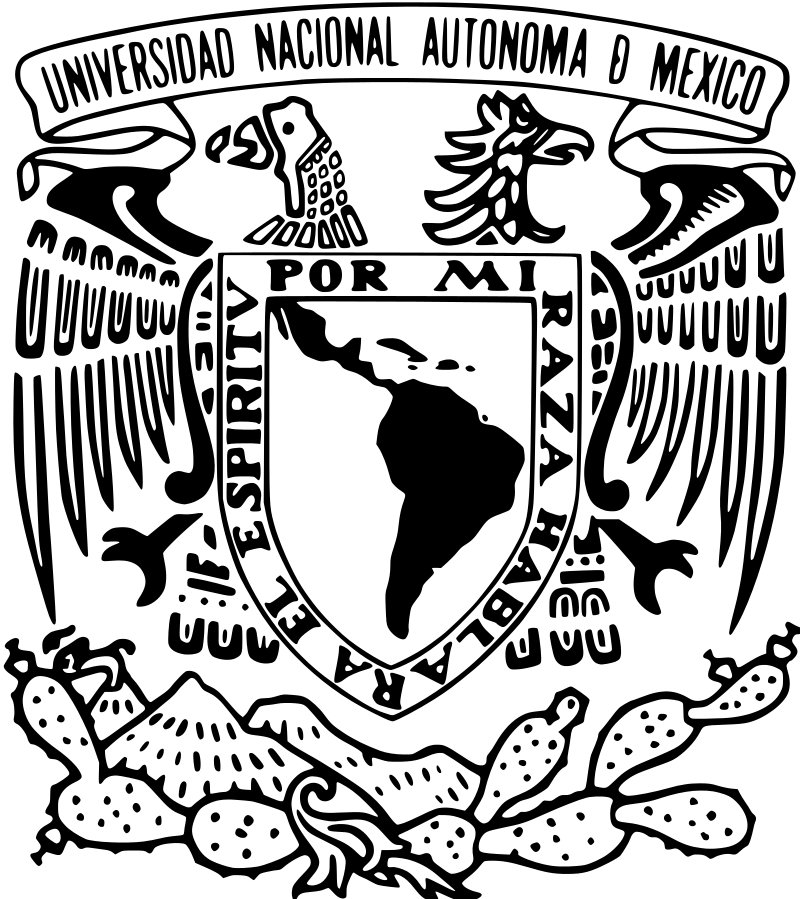
\includegraphics[width=4cm]{escudoUNAM_negro.png}
		% };

		\node[anchor=north east, inner sep=30] at (current page.north east) {
			
\includegraphics[width=3.5cm, height=4cm]{escudoFI_color.png}
		};
		% \node[anchor=north east, inner sep=30] at (current page.north east) {
		% 	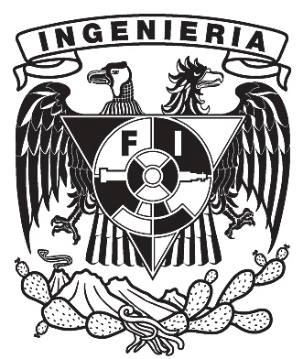
\includegraphics[width=4cm]{escudoFI_negro.png}
		% };
	\end{tikzpicture}

	\begin{center}
		\vspace*{2.5cm}

		\Large
		\textbf{UNIVERSIDAD NACIONAL AUTÓNOMA DE MÉXICO}\\
		\textbf{FACULTAD DE INGENIERÍA}\\
		\textbf{INGENIERÍA EN COMPUTACIÓN}\\

		\vspace*{1.5cm}
		\large
		\textbf{Laboratorio de Organización y Arquitectura de Computadoras}\\
		\large
		\vspace*{1cm}
		\textbf{Reporte - Construcción de Máquinas de estados Usando Memorias con Direccionamiento Implícito}\\
		\vspace{1.5cm}
	\end{center}

	%grupo de la materia
	\large
	\textbf{INTEGRANTES EQUIPO 8:}
	\begin{itemize}
		\item Saldaña Navarrete Andrea - \textit{Grupo Teoria:} 2
		\item Tepal Briseño Hansel Yael - \textit{Grupo Teoria:} 1
		\item Ugartechea González Luis Antonio - \textit{Grupo Teoria:} 1
	\end{itemize}
	\vspace{2.5cm}

	\large
	%fecha de entrega
	\textbf{NOMBRE DELPROFESOR:} Ing. Diana Karen Pérez Pérez \\
	\textbf{GRUPO:} 06\\
	\textbf{SEMESTRE:} \underline{2027-1}\\
	\vspace{0.5cm}

	\begin{center}
		\textbf{FECHA DE ENTREGA:} 5 de noviembre del 2026\\
	\end{center}
\end{titlepage}


\section*{Objetivo}

Familiarizar al alumno en el conocimiento de construcción de máquinas de estados usando direccionamiento de memorias con el método de direccionamiento implícito.

\section*{Introducción}



\section*{Desarrollo}

\subsection*{1. Diseñe una carta ASM con las siguientes características:}

\begin{itemize}
    \item Estados: 6 hasta 16
    \item Entradas: 3
    \item Salidas: 4
    \begin{itemize}
        \item 2 con lógica estándar
        \item 2 con lógica negada
    \end{itemize}
    \item Colocar al menos 3 salidas condiciones si se puede.
\end{itemize}

\begin{figure}[H]
    \centering
    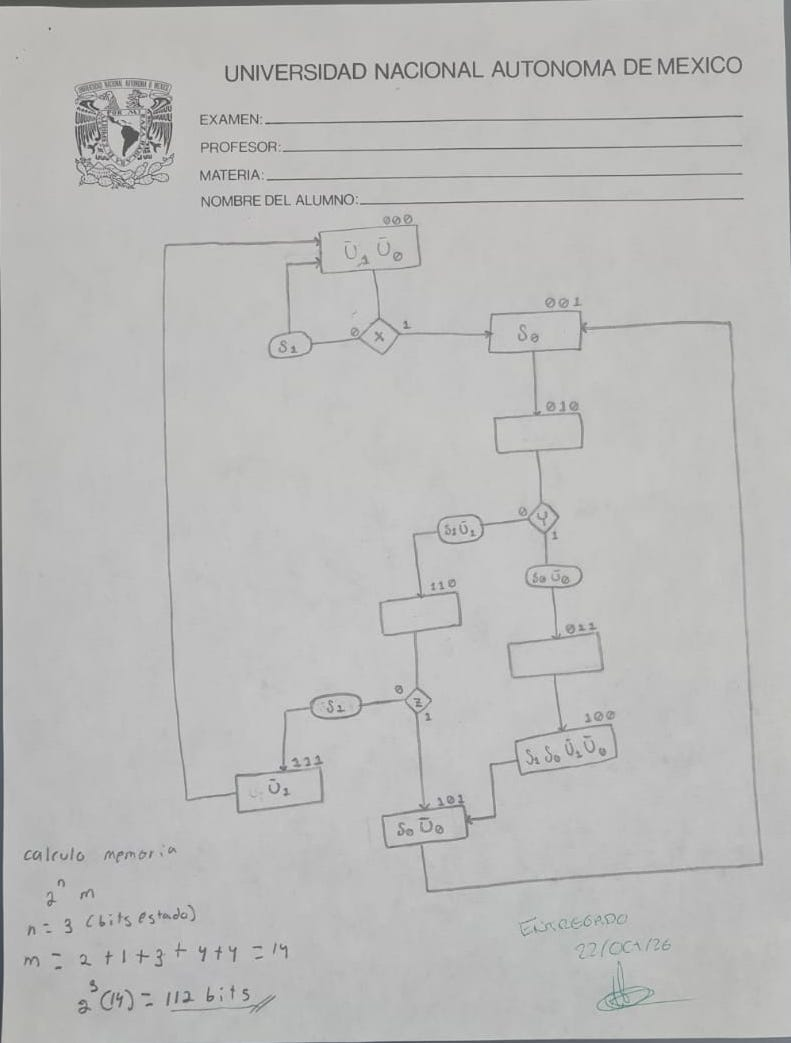
\includegraphics[width=\textwidth]{firmado.jpeg}
    \caption{Carta ASM firmada por la profesora.}
    \label{fig:carta_asm_10_limpia_firmada}
\end{figure}

\begin{figure}[H]
    \centering
    \begin{adjustbox}{width=\textwidth}
    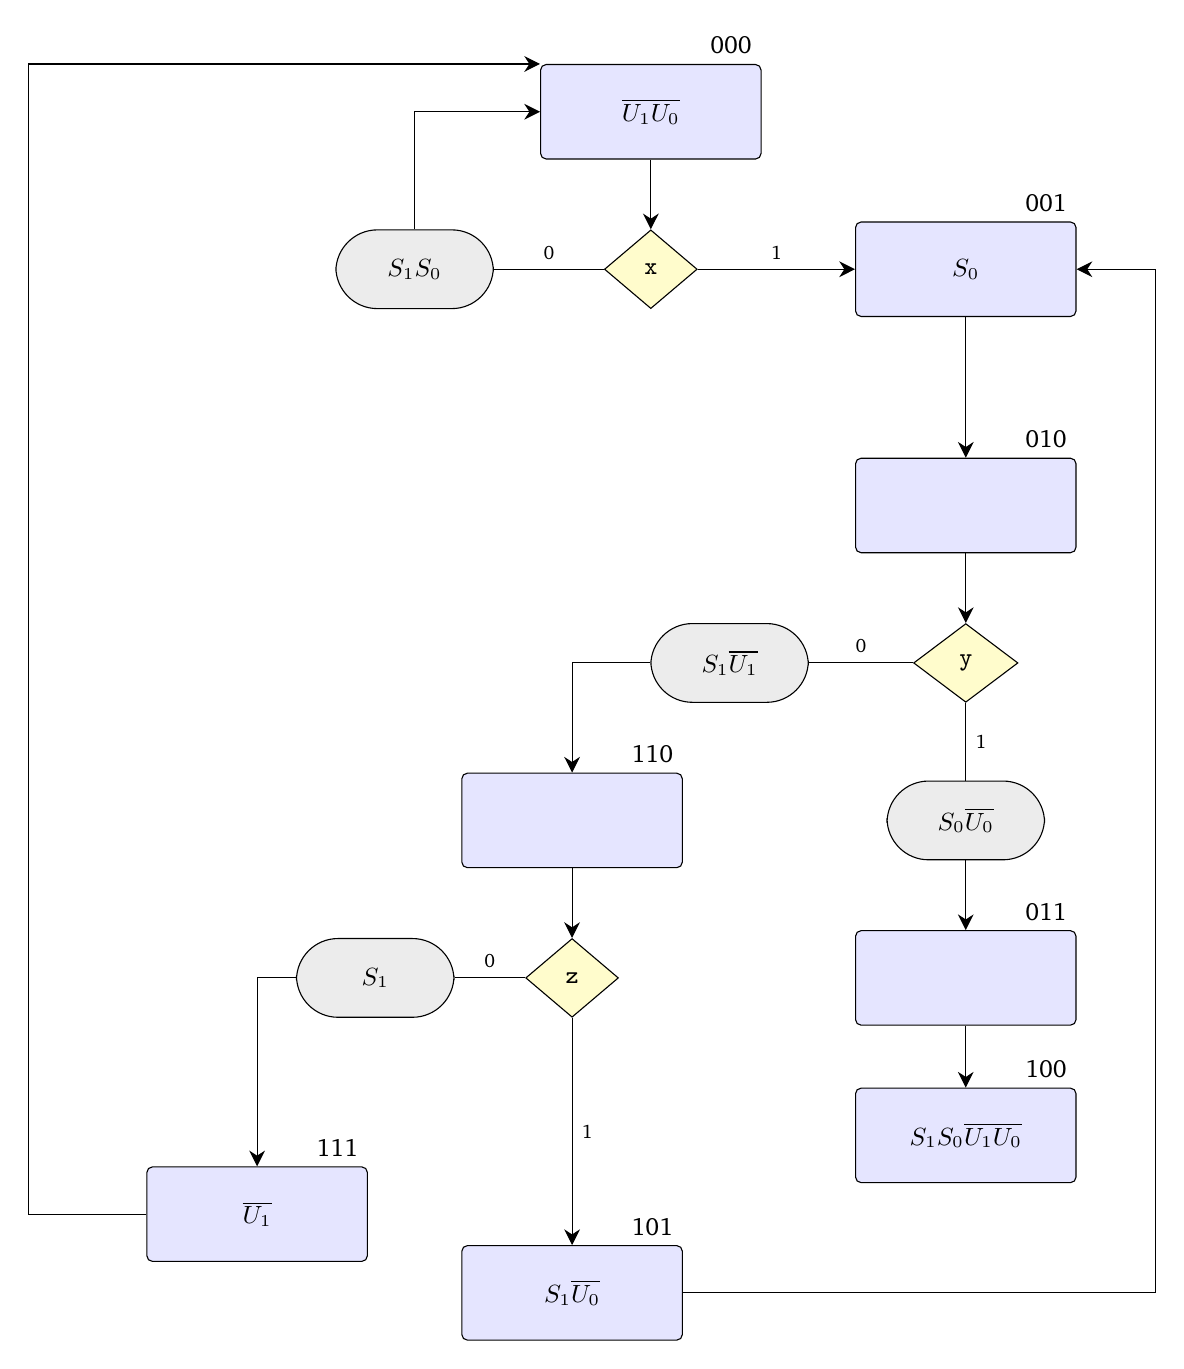
\begin{tikzpicture}[
        state/.style={draw, rounded corners=2pt, fill=blue!10, minimum width=2.8cm, minimum height=1.2cm, align=center, font=\small},
        decision/.style={draw, diamond, aspect=2.1, fill=yellow!20, minimum width=1cm, minimum height=1cm, align=center, font=\small},
        output/.style={draw, rounded corners=15pt, fill=gray!15, minimum width=2cm, minimum height=1cm, align=center, font=\small},
        >={Stealth[length=2mm,width=2mm]}
    ]
        \node[state, label={[anchor=south east, font=\small]north east:{000}}] (E0) at (0,0) {$\overline{U_1}\overline{U_0}$};
        \node[decision] (X0) at (0,-2) {\texttt{x}};
        \node[output] (C0) at (-3,-2) {$S_1S_0$};
        \node[state, label={[anchor=south east, font=\small]north east:{001}}] (E1) at (4,-2) {$S_0$};
        \node[state, label={[anchor=south east, font=\small]north east:{010}}] (E2) at (4,-5) {};
        \node[decision] (X1) at (4,-7) {\texttt{y}};
        \node[output] (C1) at (4,-9) {$S_0\overline{U_0}$};
        \node[output] (C2) at (1,-7) {$S_1\overline{U_1}$};
        \node[state, label={[anchor=south east, font=\small]north east:{011}}] (E3) at (4,-11) {};
        \node[state, label={[anchor=south east, font=\small]north east:{100}}] (E4) at (4,-13) {$S_1S_0\overline{U_1}\overline{U_0}$};
        \node[state, label={[anchor=south east, font=\small]north east:{110}}] (E6) at (-1,-9) {};
        \node[decision] (Z1) at (-1,-11) {\texttt{z}};
        \node[output] (C3) at (-3.5,-11) {$S_1$};
        \node[state, label={[anchor=south east, font=\small]north east:{111}}] (E7) at (-5,-14) {$\overline{U_1}$};
        \node[state, label={[anchor=south east, font=\small]north east:{101}}] (E5) at (-1,-15) {$S_1\overline{U_0}$};

        \draw[->] (E0) -- (X0);
        \draw[] (X0) -- node[above, font=\scriptsize] {0} (C0);
        \draw[->] (C0) |- (E0);
        \draw[->] (X0) -- node[above, font=\scriptsize] {1} (E1);
        \draw[->] (E1) -- (E2);
        \draw[->] (E2) -- (X1);
        \draw[] (X1) -- node[right, font=\scriptsize] {1} (C1);
        \draw[] (X1) -- node[above, font=\scriptsize] {0} (C2);
        \draw[->] (C1) -- (E3);
        \draw[->] (E3) -- (E4);
        \draw[->] (C2) -| (E6);
        \draw[->] (E6) -- (Z1);
        \draw[] (Z1) -- node[above, font=\scriptsize] {0} (C3);
        \draw[->] (Z1) -- node[right, font=\scriptsize] {1} (E5);
        \draw[->] (C3) -| (E7);
        \draw[->] (E7.west) -- ++(-1.5,0) |- (E0.north west);
        \draw[->] (E5.east) -- ++(+6,0) |- (E1);
        % \draw[->] (E9.east) -- ++(1,0) |- (E1.east);
    \end{tikzpicture}
    \end{adjustbox}
    \caption{Carta ASM de 8 estados con direccionamiento Implícito.}
    \label{fig:carta_asm_10_limpia}
\end{figure}

\subsubsection*{2. Encuentre el tamaño de la memoria necesaria y el contenido de memoria utilizando el direccionamiento entrada-estado.}

Encuentre el tamaño de la memoria necesaria y el contenido de memoria utilizando el direccionamiento por trayectoria. Recuerde que antes de construir la tabla se debe asignar a cada estado de la carta ASM una representación binaria. Así mismo, recuerde que para cada estado es necesario considerar todas las posibles combinaciones de las variables de entrada, aun cuando algunas de ellas no se utilicen en determinado estado.

\subsection*{Cálculo del tamaño de memoria}


\begin{figure}[H]
    \centering
    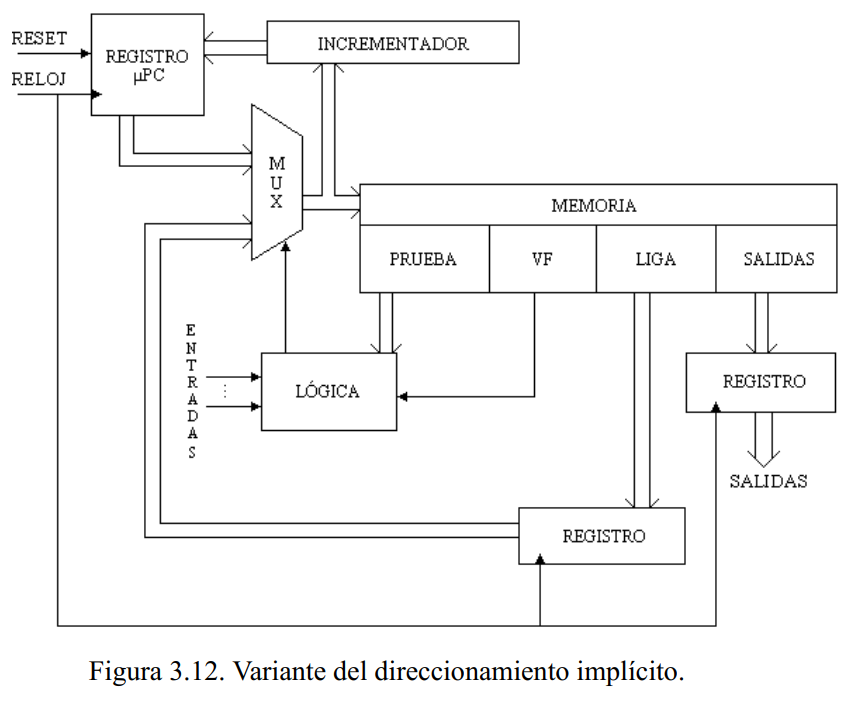
\includegraphics[width=0.7\textwidth]{diagramaImplicitoModificado.png}
    \caption{Esquema del Direccionamiento Implícito.}
    \label{fig:diagrama_modificado}
\end{figure}

\textbf{Tamaño de memoria}

\[
2^n \cdot m
\]

En donde:
\begin{itemize}
    \item $n$ = número de bits del estado presente.
    \item $m$ = prueba + liga falsa + liga verdadera + salida falsa + salida verdadera.
\end{itemize}

En esta máquina se tienen 10 estados. Por lo tanto, se necesitan 4 bits para representarlos, ya que $2^4=16$ combinaciones posibles.

\[
n = 4\text{ bits}
\]

La dirección de memoria tendrá 4 bits y podrá seleccionar 16 localidades. Para calcular la longitud de la palabra ($m$), se suman los bits de los campos requeridos por la arquitectura:

\begin{itemize}
    \item \textbf{Prueba:} 2 bits (para seleccionar entre las entradas $w=00, x=01, y=10, z=11$).
    \item \textbf{Liga Falsa:} 4 bits (estado siguiente si la evaluación es 0).
    \item \textbf{Liga Verdadera:} 4 bits (estado siguiente si la evaluación es 1).
    \item \textbf{Salida Falsa:} 4 bits (estado de las salidas $S_1, S_0, \overline{U_1}, \overline{U_0}$ si la evaluación es 0).
    \item \textbf{Salida Verdadera:} 4 bits (estado de las salidas si la evaluación es 1).
\end{itemize}

\[
m = 2 + 4 + 4 + 4 + 4 = 18\text{ bits}
\]

Por lo tanto, el tamaño de memoria necesario es:

\begin{tcolorbox}[colback=gray!20,colframe=LimeGreen!75!black]
\[
2^4\cdot 18 = 16\cdot 18 = 288\text{ bits}
\]
\end{tcolorbox}

\subsection*{Contenido de la memoria}


\subsection*{3. Implementación en Quartus del direccionamiento implícito.}

Una vez que haya obtenido el contenido de memoria, implemente el direccionamiento implícito utilizando el software de desarrollo Quartus y escriba el contenido de memoria obtenido.

% \subsubsection*{Divisor de Frecuencia (\texttt{div\_frec.vhd})}

\subsection*{4. Modifique el código de Quartus para que se acepten salidas condicionales.}

\section*{Discusión de Resultados}

\subsection*{5. Simule su diseño para probar su funcionamiento. Recuerden que en sus simulaciones debe aparecer el contenido de la memoria además del estado presente.}

\subsubsection*{Simulación 1}



\subsubsection*{Simulación 2}


\subsubsection*{Simulacion 3}



\section*{Conclusiones}

\subsection*{Andrea Saldaña Navarrete - 320206384}



\subsection*{Hansel Yael Tepal Briseño - 320078282}



\subsection*{Luis Antonio Ugartechea González - 320223822}



\newpage
\section{Bibliografía}

% En formato IEEE

\begin{biblio}
	\hypertarget{1-diana-karen}{}
	\item D. K. Pérez Pérez, ``Reporte Construcción de Máquinas de Estados Usando Memorias'', Laboratorio de Organización y Arquitectura de Computadoras, Facultad de Ingeniería, Universidad Nacional Autónoma de México, Semestre 2027-1, 2026.
	\hypertarget{2-facultad-ingenieria}{}
	\item Facultad de Ingeniería, ``Capítulo III: Construcción de máquinas de estados usando memorias'', Apuntes de Arquitectura de Computadoras, Universidad Nacional Autónoma de México (UNAM). [En línea]. Disponible en: \url{https://biorobotics.fi-p.unam.mx/wp-content/uploads/Courses/arquitectura_de_computadoras/2021-1/lecciones/Leccion_3_arquitectura_de_computadoras_2021_1.pdf}
	% \hypertarget{3-savage}{}
	\item J. Savage, \textit{Diseño de Microprocesadores}, Facultad de Ingeniería, Universidad Nacional Autónoma de México (UNAM). [En línea]. Disponible en: \url{http://profesores.fi-b.unam.mx/luist/archivos/MicroprocesadoresSavage.pdf}
\end{biblio}

\end{document}
